\documentclass[mathserif,serif]{beamer}

\usepackage{graphicx}
\graphicspath{ {images/} }

\title
{Brain Viewer Review}
\subtitle{Current situation and the next steps}
\author
{Pierpaolo Rametta}

\subject{SPINE' s Tool}

\usetheme{Warsaw}

\begin{document}
  \frame{\titlepage}

  \begin{frame}
    \frametitle{What we can do}
    	\begin{itemize}
    		\item Load brain model in .asc format using brainbrowser framework
    		\item Click on a vertex and retrieve the relative region
    		\item Select .nii file
    		\item Check for multiple regions and perform the search on the selected .nii
    		\item Display and save the slices in which the regions are present
    	\end{itemize} 

  \end{frame}

  \begin{frame}
  	\frametitle{What we can do}

  	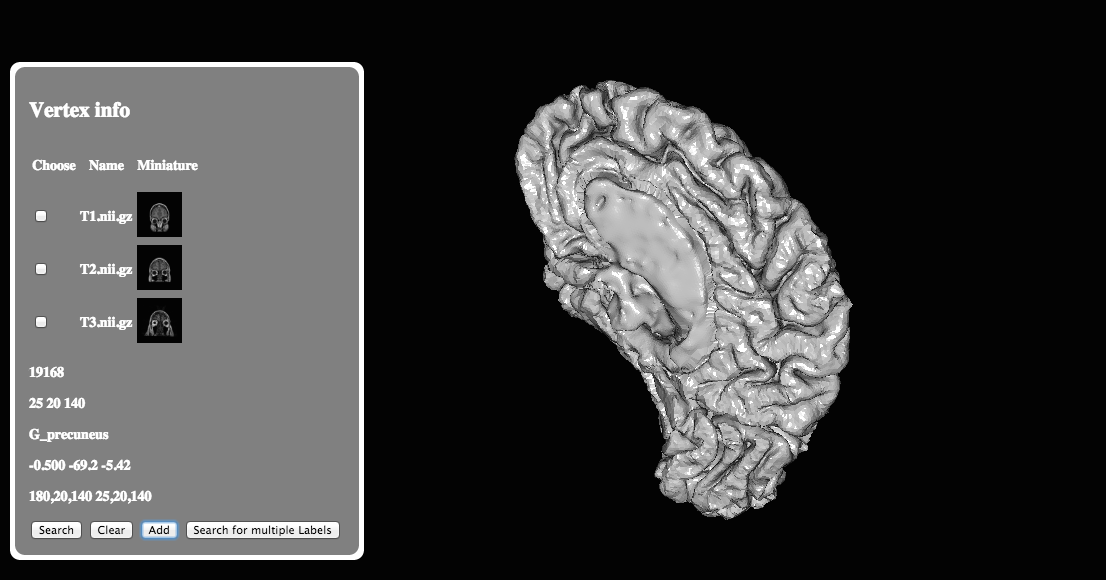
\includegraphics[width=10.5cm, height=5cm]{screenshot1}

  \end{frame}

  \begin{frame}
    \frametitle{Interaction with the server}
    \framesubtitle{What we have on the server side}

    	\begin{itemize}
    		\item Nifti files and their segmented parts 
    		\item We use the aparc.annot.a2009s.ctab file to retrieve the id foreach vertex according to freesurfer standards
    		\item User libs to perform searches  
    	\end{itemize}

  \end{frame}

  \begin{frame}
  	\frametitle{The next steps}

  		\begin{itemize}
  			\item Modify the code to use Angular and Hapi frameworks
  			\item Adding AND - OR interrogations
  			\item Modify slice deleting pixel that does not contain a given value
  			\item Other interrogations types
  		\end{itemize}
  \end{frame}

\end{document}